\chapter{Strehl Calculation Tool}

\section{Description}

An adaptive optics system compensates phase errors to return the resolution of the system to the diffraction limit of the telescope. The correction is not perfect, and we are interested in measuring the performance of the AO system. The Strehl ratio is defined as the ratio between the peak of an imaged PSF, with the peak of an aberration-free PSF. The Strehl ratio can be used to approximate the residual RMS uncorrected phase errors through the Marechal approximation given by:

\begin{equation}
    S \cong e^{-\sigma^2}
\end{equation}

where $S$ is the Strehl ratio, and $\sigma^2$ is the phase variance of the wavefront in units of radians. The measurement of the Strehl ratio for an AO corrected PSF is given in Equation \ref{Strehl}. The Strehl ratio is calculated by taking the ratio of the peak intensity of the partially corrected PSF, $P_{data}$,  to the peak intensity of an aberration free PSF, $P_0$. The peaks are normalized by the flux in the image. A simulated model can be used for the aberration free image. 

\begin{equation}
    S=\frac{P_{data}/Flux_{data}}{P_{0}/Flux_{0}}
    \label{Strehl}
\end{equation}

The calculation of Strehl for the data taken from the CACTI testbed was done using a Strehl ratio calculation tool that developed in Python. The flow of the Strehl ratio code is given in Figure \ref{fig:strehlClass}. The user inputs a list of filenames containing the image files (pathToData) and the image file for the aberration free PSF (pathToPerfect). For the CACTI testbed our aberration free PSF was the flat wavefront PSF on the science camera created by the deformable mirror, which we will refer to as the reference PSF. A simulated perfect PSF matching the plate scale of the system is an alternative. These two paths are the only mandatory inputs to the pipleline. If only one filename is given in pathToPerfect, then that reference PSF will be used in the Strehl calculation for every data file. If multiple files are used for the reference PSF, than the number of filenames for pathToPerfect must match that of pathToData. In this case, the reference PSF will be used with the data PSF from the filename with the same list index to calculate Strehl. An optional file to read in is pathToDarks which contains the dark files that will be used in dark subtraction. For CACTI the same camera is used to record the AO corrected PSFs and the reference PSF so the dark file is the same and used for both data sets. The pipleline checks that none of the data is saturated, by comparing the max of every image to the hard coded over-saturation value of the science camera which is a value 1023. If any of the data is over-saturated the pipeline with produce an error.

The Strehl ratio is calculated using the peak of the data. The Strehl calculation tool can find the peak of each image two different ways. The default method assumes that the highest value in each image is the peak of the data. An optional way is to use the Smart Peak Finder, which is an optional attribute provided by the user. The Smart Peak Finder uses the DAOStarFinder from Astropy that uses a Gaussian fitter to find the peak of the image. The user can provide the full-width half-max (FWHM) of the Gaussian kernel used by DAOStarFinder as an optional object attribute. If the user does not specify a FWHM, the Strehl Calculation tool will estimate the FWHM by pulling a sample image from the reference PSF data, and fitting a Gaussian to the a slice of the PSF created by taking the radial average around the max value in the frame. Once the peak value in each frame is found, the coordinates of that peak are saved for later use in the pipeline. 

The dark subtraction is performed in two steps. First if the user provided a dark files, they are subtracted off of frame. A second round of dark subtraction is done by masking out the PSF, and row by row taking the average value of the row, and subtracting it from that row. The mask is a circular mask centered on the coordinates of the peak found in the previous step. There is a default diameter to the mask which is one third the size of the smallest dimension of the images. A diameter can be provided as an optional input by the user. After dark subtraction the peak value is then pulled from every frame to be used in the Strehl calculation detailed in Equation \ref{Strehl}. The peak is normalized by the Flux in the image. To do this the Strehl Calculation tool sums the Flux in circles of increasing radii that are centered on the peak of the image. The result is a Strehl as a function of radius from the peak. Figure \ref{fig:StrehlVsRadiiExample} is a plot of the output from the Strehl Calculator tool, for a data set of closed loop PSFs from five different files, each file representing a single closed loop run. The turbulence strength for this data set was 0.3 microns RMS. As the radii of the summed Flux increases, the Strehl ratio flattens out which indicates a good background subtraction was done. If the background subtraction was poor, the Strehl ratio would increase as radius increased. Making the diameter of the PSF mask used for background subtraction smaller can help solve this issue. 

\begin{figure}
    \centering
    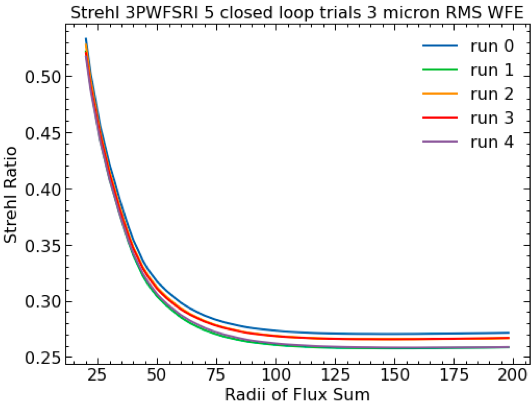
\includegraphics[width=0.8\textwidth]{Chapter Materials/Appendix Materials/StrehlVsRadiiExample.png}
    \caption{Out put of the Strehl calculation tool. For each filename given, the data in the file is used to calculate a mean Strehl value. The value is plotted again the radius of the circle used to sum the Flux for normalization. Having the Strehl value converge to a flat value as shown, is an indicator that the background subtraction was done correctly. }
    \label{fig:StrehlVsRadiiExample}
\end{figure}


\begin{figure}
    \centering
    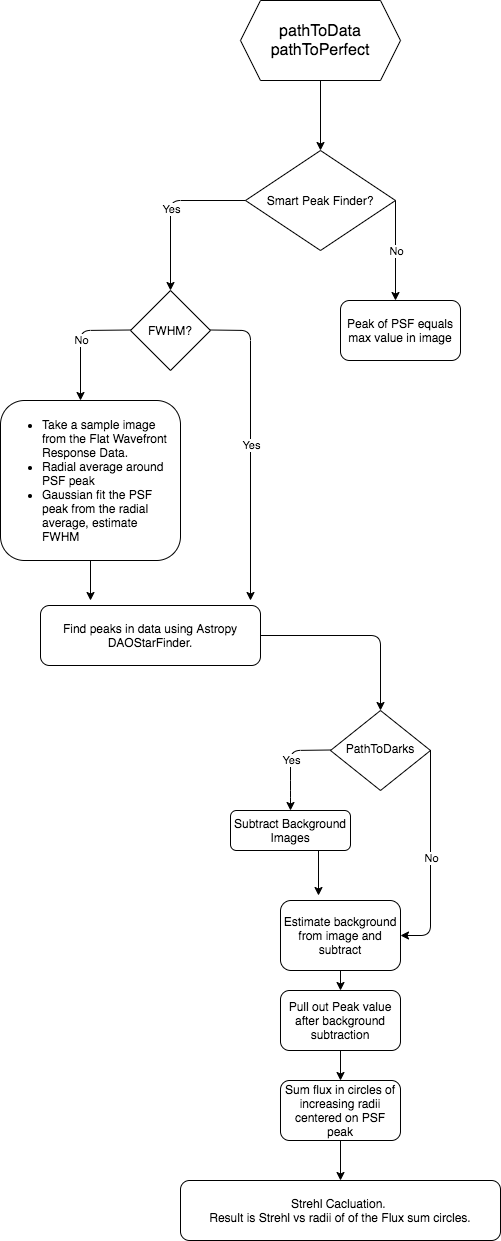
\includegraphics[scale=0.4]{Chapter Materials/Appendix Materials/strehlclass2.png}
    \caption{Flow and decision tree of the Strehl calcualation tool. The Strehl can be calculated two ways. One way assumes that the max value in the image is the peak of the PSF. The second way is smarter, and uses DAOStarFinder tool from Astropy that uses a Gaussian fitter to find the peak of the image. The final product is Strehl as a function of the radius of the circle used to sum the Flux for normalization. }
    \label{fig:strehlClass}
\end{figure}

\newpage

\section{Code}
\begin{lstlisting}
from astropy.io import fits
import numpy as np
import matplotlib.pyplot as plt
from photutils import DAOStarFinder
from astropy.stats import sigma_clipped_stats
from astropy.modeling import models, fitting



class strehlCalc:   

        
# ###### Current attributes:

# User inputs upon object creation: ------------------------

# All data should be .fits files
    
# All paths must be in a list!
    # ex) 
        #pathToData=[None]*N
        #pathToData[0]='path'
    
#     pathToData:     Path where the image data of the closed loop PSFs are stored. Each .fits file should have one data cube of image frames.

#     pathToFlats:    path where the PSF response to a flat wavefront is stored.                      
#                     This is what the closed loop PSFs are compared to in the Strehl calculation

#     pathToDarks:    If you have a dark image, input the path.
#                     Can be a single frame (Hopefully a mean frame from multiple dark frames), 
#                     or a data cube of individual dark frames that will be averaged for you.
#                     If not, the background will be estimated from the image frame.

#     drkSubtractDiameter:     
#                     Diameter in pixels of the circular mask that masks out the PSF 
#                     for the dark subtraction that is estimated from the image frame. 
#                     * A common fix to a bad strehl measurement is decreasing the diameter size. 
#                     If none is given the diameter of the mask will be 1/3 the smallest dimension of the data frame . 

# Class generated attributes: --------------------------

## Saturation check. Each index corresponds to the file opened in the list pathTo... with the same index.

### The saturated value for the Basler Cameras is 1023, and is a hard coded value. If your camera has a different saturation value change it in code. 

#     darkSat:        True: dark data is oversaturated. False: dark data is not saturated
#     imageSat:       True: there are one or more frames in that file that are oversaturated. False: no frames in that file are oversaturated.
#     perfSat:        True: there are one or more frames in that file that are oversaturated. False: no frames in that file are oversaturated. 


#     imagePeak:      The peak values of the PSF used in Strehl Calculation
#     perfPeak:       The peak values of the perfect PSF the closed loop PSFs will be compared to in the Strehl Calculation
#     imgFlux:        The sum of the flux values of the PSF used in the Strehl Calculation. The flux is summed over circles of increasing diameter. 
#     perfFlux:       The sum of the flux values of the perfect PSF the closed loop PSFs will be compared to in the Strehl Calculation. The flux is summed over circles of increasing diameter.
#     fluxDiameter:   The diameters in pixels that the flux was summed over.

#     imageSize:      Size of the data cube containing the closed loop PSF data
#     perfSize:       Sixe of the data cube containing the images of the flat wavefront response PSF data

#     self.Strehl:    The calculated Strehl ratio for each image file, at each 

        

    
    def __init__(self, pathToData,pathToFlats, pathToDarks=None,FWHM=None, smartPeak=None,drkSubtractDiameter=None):
        self.pathToData=pathToData
        self.pathToFlats=pathToFlats
        if pathToDarks:
            self.pathToDarks=pathToDarks
            self.darkSat, self.darkData, self.darkSize=self.openFile(self.pathToDarks)
        else:
            pathToDarks=None
            self.darkSat=False 
            
        #open the files, test if any are oversaturated  
        self.imageSat, imageData, self.imageSize=self.openFile(self.pathToData)
        self.perfSat, perfData, self.perfSize=self.openFile(self.pathToFlats)
            
        ## Check to make sure the data is not oversaturated and compatible with the pipeline. 
        self.errorMsg()
        
        if smartPeak:
            if FWHM:
               self.FWHM=FWHM 
            else:
                print("Estimating the FWHM.")
                self.radialA, self.totalProfile=self.radialAveragePrep(perfData)
                self.FWHM, self.FWHMval=self.fwhmEstimate()
            print('Finding the peak of the data using DAOStarFinder.')
            xcentroid, ycentroid=self.smartPeakFinder(imageData)
            xPerfcentroid, yPerfcentroid=self.smartPeakFinder(perfData)
                
        else:
            print('Finding the peak using the max value in data.')
            xcentroid, ycentroid=self.peakFinder(imageData) ### RETURN ONLY THE CENTROIDS
            xPerfcentroid, yPerfcentroid=self.peakFinder(perfData)
            
        
        # dark subtract + pull out image peak
        pData=self.darkSubtract(imageData,xcentroid, ycentroid)
        pPerfData=self.darkSubtract(perfData,xPerfcentroid, yPerfcentroid)
        print("Finished dark subtraction.")
        
        #Assumes the coordinates of the peak haven't changed after dark subtraction
        
        self.imagePeak=self.coord2peak(pData, xcentroid, ycentroid)
        self.perfPeak=self.coord2peak(pPerfData, xPerfcentroid, yPerfcentroid)
        print("Found the peak in each image.")
        
#       #Sum the Flux in a circle centered on the PSF at increasing radii.  
        
        self.fluxDiameters, self.imageFlux=self.sumFlux(xcentroid, ycentroid,pData)
        self.perfFluxDiameter, self.perfFlux=self.sumFlux(xPerfcentroid, yPerfcentroid, pPerfData)
        print("Summed the flux in each image.")
        
#         # Calculate the Strehl value. 
        print("Calculating the Strehl Ratio.")
        self.Strehl=self.strehlCalculator()
        print("Finished.")
        
    
    
##### Functions -------------------------------------------------------------
        
                      
    def openFile(self, path):
            
        #check if it is a single file or multiple
        fileSize=np.shape(path)
        
        ## Pull a test file
        testFile=fits.open(path[0])
        testData=testFile[0].data
        dataSize=np.shape(testData)
        
        data=np.zeros((*fileSize,*dataSize))
        oversaturated=fileSize[0]*[None]
        
        data[0,:]=testData
        oversaturated[0]=np.any(testData == 1023)
        
        # Pull out the rest of the data and check if it is oversaturated
        for i in range(fileSize[0]-1):
            i=i+1
            testFile=fits.open(path[i])
            data[i,:]=testFile[0].data
            oversaturated[i]=np.any(data[i,:] == 1023)
        
        imageSize=np.shape(data)

            
        return oversaturated, data, imageSize
                           
    
    def darkSubtract(self, data,xcentroid, ycentroid, drkSubtractDiameter=None):
        
        imageSize=np.shape(data)
        
        #takes the mean if it is a data cube
        if hasattr(self, 'darkData'):
            dkData=np.mean(self.darkData,axis=0)
            for i in range(imageSize[0]):
                data[i,:]=np.subtract(data[i,:],dkData)
            print("Subtracted Dark Frame")

        
        ## Find peak of data to center mask: Assumes the max value in image is the peak.

#         xcentroid=np.zeros((imageSize[0],imageSize[1]))
#         ycentroid=np.zeros((imageSize[0],imageSize[1]))
        
#         for i in range(imageSize[0]):
#             for j in range(imageSize[1]):
#                     max_xy=np.where(data[i,j,:,:]==data[i,j,:,:].max())
#                     xcentroid[i,j]=max_xy[1][0]
#                     ycentroid[i,j]=max_xy[0][0]
        
                
        ### Second round of background subtraction based of the image background.
        
        # Places a circle mask over the PSF data of diameter given by user input. 
        #If no user input, it uses a diameter=1/3 smallest dimension of a single data frame. 
        #After, row by row takes the mean value of the row, and subtracts it from that row. 
        
            
        if drkSubtractDiameter == None:
            check=min(imageSize[2],imageSize[3])
            drkSubtractDiameter=np.round(check/3)
        
        pData=np.zeros(imageSize)
        
        for i in range(imageSize[0]):
            for j in range(imageSize[1]):
                mask=self.circle(imageSize[2],imageSize[3],drkSubtractDiameter,xcentroid[i,j],ycentroid[i,j])
                mask=1-mask
                dummy=mask*data[i,j,:]
                for k in range(imageSize[2]):
                    m=np.mean(dummy[k,:])
                    pData[i,j,k,:]=np.subtract(data[i,j,k,:],m)
                    

            
        return pData
    
    def coord2peak(self, data, xcentroid, ycentroid):
        imageSize=np.shape(data)
        peak=np.zeros((imageSize[0],imageSize[1]))

        for i in range(imageSize[0]):
             for j in range(imageSize[1]):
                    peak[i,j]=data[i,j,int(ycentroid[i,j]),int(xcentroid[i,j])]
        
        return peak
    
    
    def peakFinder(self,data):
    #Stupid Peak finder. Pulls out the max value of the image as the peak. 
    ## Pull out the values of the PSF peak after dark subtraction
        imageSize=np.shape(data)
        xcentroid=np.zeros((imageSize[0],imageSize[1]))
        ycentroid=np.zeros((imageSize[0],imageSize[1]))
        
        
        for i in range(imageSize[0]):
            for j in range(imageSize[1]):
                max_xy=np.where(data[i,j,:,:]==data[i,j,:,:].max())
                xcentroid[i,j]=max_xy[1][0]
                ycentroid[i,j]=max_xy[0][0]
            
        return xcentroid, ycentroid
        
        
    def smartPeakFinder(self,data):
        #Smart Peak finder using photutils from the astropy package
        fwhmSize=np.shape(self.FWHM)
        imageSize=np.shape(data)
        xcentroid=np.zeros((imageSize[0],imageSize[1]))
        ycentroid=np.zeros((imageSize[0],imageSize[1]))
        
        if fwhmSize[0]==1:

            for i in range(imageSize[0]):
                sdev=np.std(data[i,:])
                daofind = DAOStarFinder(fwhm=self.FWHM[0], threshold=5.*sdev)
                for j in range(imageSize[1]):
                    sources=daofind(data[i,j,:])
                    for col in sources.colnames:
                        sources[col].info.format = '%.8g'
                        peak=max((sources["peak"]))
                        ind=np.where(sources["peak"]==max(sources["peak"]))
                        xc=(sources["xcentroid"][ind[0]])
                        yc=(sources["ycentroid"][ind[0]])     
                        xcentroid[i,j]=int(np.round(xc[0]))
                        ycentroid[i,j]=int(np.round(yc[0]))
        else:  
            for i in range(imageSize[0]):
                sdev=np.std(data[i,:])
                daofind = DAOStarFinder(fwhm=self.FWHM[i], threshold=5.*sdev)
                for j in range(imageSize[1]):
                    sources=daofind(data[i,j,:])
                    for col in sources.colnames:
                        sources[col].info.format = '%.8g'
                        peak=max((sources["peak"]))
                        ind=np.where(sources["peak"]==max(sources["peak"]))
                        xc=(sources["xcentroid"][ind[0]])
                        yc=(sources["ycentroid"][ind[0]])     
                        xcentroid[i,j]=int(np.round(xc[0]))
                        ycentroid[i,j]=int(np.round(yc[0]))
                        
        return xcentroid, ycentroid


    def fwhmEstimate(self):
        from astropy.modeling import models, fitting 
        s=np.round(len(self.totalProfile[0,:])/2)
        x=np.arange(-s+1,s,1)
        
        sz=np.shape(self.totalProfile)
        FWHM=np.zeros(sz[0])
        FWHMval=np.zeros(sz[0])
        
        #fit Guassian to data
        for i in range(sz[0]):
            g_init = models.Gaussian1D(amplitude=1., mean=0, stddev=1)
            fit_g = fitting.LevMarLSQFitter()
            g = fit_g(g_init, x, self.totalProfile[i,:])
            
            gaus=g(x)
            stdv=np.std(gaus)
            FWHMval[i]=2*np.sqrt(2*np.log(2))*stdv
            
            val=gaus[gaus>=FWHMval[i]]
            FWHM[i]=len(val)
            
        return FWHM, FWHMval
            
            
    
    def radialAveragePrep(self,data):
        
        #calculates an estimated radial average in one frame of data per file. 
        #This is meant to be passed to the Full width half max estimator.
        
        imageSize=np.shape(data)
        xcentroid=np.zeros((imageSize[0]))
        ycentroid=np.zeros((imageSize[0]))
        
        for i in range(imageSize[0]):
            max_xy=np.where(data[i,0,:,:]==data[i,0,:,:].max())
            xcentroid[i]=max_xy[1][0]
            ycentroid[i]=max_xy[0][0]
        
        
        if imageSize[2] != imageSize[3]:
            check=min(imageSize[2],imageSize[3])
            radData=np.zeros(imageSize[0],1,check, check)
            for i in range(imageSize[0]):
                radData[i,0,:]=self.cropper(data[i,0,:,:],xcentroid[i], ycentroid[i], check)
        else:
            radData=np.zeros((imageSize[0],1,imageSize[2],imageSize[3]))
            for i in range(imageSize[0]):
                radData[i,0,:,:]=data[i,0,:,:]
                
        
        test=self.radial_data_median_only(radData[0,0,:,:],1)
        radSize=np.shape(test)
        radialA=np.zeros((imageSize[0],radSize[0]))
        totalProfile=np.zeros((imageSize[0],radSize[0]*2-1))
        for i in range(imageSize[0]):
            radialA[i,:]=self.radial_data_median_only(radData[i,0,:,:],1)
#             m=np.mean(radialA[i,0:100])
#             radialA[i,:]=radialA[i,:]-m
            flip=np.flip(radialA[i,:])
            totalProfile[i,:]=np.concatenate((flip, radialA[i,1:]))
        
        return radialA, totalProfile
        
  
        
    
    def sumFlux(self, xcentroid, ycentroid, data):
        
        
        imageSize=np.shape(data)
        check=min(imageSize[2],imageSize[3])
        x=np.floor(np.floor(((np.floor((check/10))*10)))/10)*10-50
        r1=range(20, int(x), 2)
        sz2=np.shape(r1)
        rFlux=np.zeros((imageSize[0],imageSize[1],sz2[0]))
        
        for j in range(imageSize[0]):
            count=0
            for r in r1:
                for i in range(imageSize[1]):
                    mask=self.circle(imageSize[2],imageSize[3], r, xcentroid[j,i], ycentroid[j,i])
                    mData=data[j,int(i),:,:]*mask
                    rFlux[j,int(i),count]=np.sum(mData)
                count=count+1 
        
        return r1, rFlux   
        
    def strehlCalculator(self):   
        #if only one data cube is given use it for all frames
        #if the same number of data cubes are given match the PSFs to the same index as the corresponding Flat
        
        # if there is a corresponding flat wavefront PSF data cube to each of the closed loop PSF data cubes
        
        if self.perfSize[0]>1:
            
            sz=np.shape(self.imageFlux)
            Strehl=np.zeros((sz[0],sz[2]))
            for i in range(sz[0]): 
                for j in range(sz[2]):  
                    d=np.mean(self.imagePeak[i,:]/self.imageFlux[i,:,j])
                    p=np.mean((self.perfPeak[i,:]/self.perfFlux[i,:,j]))
                    Strehl[i,j]=d/p
                    
        
        # if there is a single flat wavefront PSF data cube corresponding to all of the closed loop PSF data cubes
        if self.perfSize[0]==1:
            print("I am using the same reference PSF to calculate Strehl for all data sets.")
            sz=np.shape(self.imageFlux)
            Strehl=np.zeros((sz[0],sz[2]))

            for i in range(sz[0]): 
                for j in range(sz[2]):  
                    d=np.mean(self.imagePeak[i,:]/self.imageFlux[i,:,j])
                    p=np.mean(self.perfPeak[0,:]/self.perfFlux[0,:,j])
                    Strehl[i,j]=d/p
        
        return Strehl
        
    def circle(self,s,v,d,x,y):
        s=s+1
        v=v+1
        cen=np.array([x,y])
        r=np.zeros([s,v])
        a=np.arange(-cen[0]+1,v-cen[0],1)
        b=np.arange(-cen[1]+1,s-cen[1],1)
        [X,Y]=np.meshgrid(a,b)
        r=np.sqrt(np.double((X**2+Y**2)))
        c = (r<=d/2).astype(int)
        return c
        
        
    def errorMsg(self):
        
        if self.perfSize[0]>1 and self.perfSize[0] != self.imageSize[0]:
            print("Error: The flat wavefront PSF data frames must be either a single data cube, or a number of data cubes equalling the number of closed loop PSF data cubes.")
            raise ValueError
        if self.imageSat == True:
            print("One or more of the closed loop PSF data frames is oversaturated.")
            raise ValueError
        if self.perfSat == True:
            print("One or more of the flat wavefront PSF data frames is oversaturated.")
            raise ValueError
        if self.darkSat == True:
            print("One of more of the dark frames is oversaturated.")
            raise ValueError
                           
    def radial_data_median_only(self,data,annulus_width=1,working_mask=None,x=None,y=None,rmax=None):
    #Pared down version of radial_data that computes only the median radial profile
        data = np.array(data)
    
        if working_mask==None:
            working_mask = np.ones(data.shape,bool)
    
        npix, npiy = data.shape
        if x==None or y==None:
            x1 = np.arange(-npix/2.,npix/2.)
            y1 = np.arange(-npiy/2.,npiy/2.)
            x,y = np.meshgrid(y1,x1)

        r = abs(x+1j*y)

        if rmax==None:
            rmax = r[working_mask].max()

        dr = np.abs([x[0,0] - x[0,1]]) * annulus_width
        radial = np.arange(rmax/dr)*dr + dr/2.
        nrad = len(radial)
        #radialdata = radialDat()
        radialdata_median = np.zeros(nrad)

        for irad in range(nrad): #= 1:numel(radial)
            minrad = irad*dr
            maxrad = minrad + dr
            thisindex = (r>=minrad) * (r<maxrad) * working_mask
            if not thisindex.ravel().any():
                radialdata_median[irad] = np.nan
            else:
                radialdata_median[irad] = np.nanmedian(data[thisindex])
    
        return radialdata_median
                           
    def cropper(self,data, x, y, d):
    ## takes the imput matrix (data) and crops a dxd square around the coordinate (x,y). Returns the cropped image

        box=pData[y-d:y+d,x-d:x+d]
        return box
            
\end{lstlisting}


\chapter{OOMAO Code}\label{OOMAOcode}

Chapter \ref{CH4} discusses changes made to the OOMAO code to enable Raw Intensity signal processing and the 3PWFS. This appendix lists the code for key parts of that work. Section \ref{mask} is the code developed to create the phase screens that simulate the pyramid optic. Section \ref{slopescode} is the code that does the signal processing. In this code the Slopes Maps are calculated, or alternatively the pixels that have signal are selected for Raw Intensity. Lastly, Section \ref{oomaoexamp} is an example experimental script for generating the AO objects, and closing the AO loop in OOMAO. 

\section{Mask Generation Code}\label{mask}
\lstset{language=Matlab}
\begin{lstlisting}

        %% make the pyramid phase mask
        function makePyrMask(pwfs)
            

if pwfs.alternative == 0
            nFaces_ = pwfs.nFaces;
            nx      = pwfs.pxSide;
            ny      = nx;
            %pwfs.rotation=0;
            
            cx = pwfs.pxSide/2+0.5;
            cy = cx;
            
            %x = linspace(-cx+1, nx-cx, nx);%*pi/sqrt(2);
            %y = linspace(-cy+1, ny-cy, ny);%*pi/sqrt(2);
            %[xGrid, yGrid] = meshgrid(x, y);
            [xGrid,yGrid]=freqspace(pwfs.pxSide,'meshgrid');
            xGrid = xGrid.*floor(pwfs.pxSide/2);
            xGrid=xGrid.*pwfs.alpha.*2/sqrt(2);
            yGrid = yGrid.*floor(pwfs.pxSide/2);
            yGrid=yGrid.*pwfs.alpha.*2/sqrt(2);

            % DEFINE THE SLOPE GRID for the mask
            angleGrid = atan2(yGrid*sin(pwfs.rotation) + ...
                xGrid*cos(pwfs.rotation), ...
                yGrid*cos(pwfs.rotation) - ...
                xGrid*sin(pwfs.rotation));

            
            % INITIALIZE PYRAMID MASK
            pyp = zeros(nx, ny);
            s1=zeros(nx,ny);
            s2=zeros(nx,ny);
            s3=zeros(nx,ny);
            for kFaces=0:nFaces_-1
                theta = (pi*(1/nFaces_ - 1) + kFaces*2*pi/nFaces_ + pwfs.rotation);
                slope = (sin(theta)*xGrid + cos(theta)*yGrid);
                %Take into account the last tile of the pyramid mask
                if kFaces == nFaces_-1
                 
                    slope((-pi+kFaces*2*pi/nFaces_ <= angleGrid) &...
                        (angleGrid <= (-pi+(kFaces + 1)*2*pi/nFaces_))) = 1; 
                    
                    s3((-pi+kFaces*2*pi/nFaces_ <= angleGrid) &...
                        (angleGrid < (-pi+(kFaces + 1)*2*pi/nFaces_))) = 1;
                        
                else
                   
              slope((-pi+kFaces*2*pi/nFaces_ <= angleGrid) &...
                        (angleGrid <= (-pi+(kFaces + 1)*2*pi/nFaces_))) = 1;
                    if kFaces==0
                    s1((-pi+kFaces*2*pi/nFaces_ <= angleGrid) &...
                        (angleGrid <= (-pi+(kFaces + 1)*2*pi/nFaces_))) = 1;
                    end
                    if kFaces==1
                        s2((-pi+kFaces*2*pi/nFaces_ <= angleGrid) &...
                        (angleGrid <= (-pi+(kFaces + 1)*2*pi/nFaces_))) = 1;
                    end
                end
            
            pyp = pyp+slope;
            end
                
pyp=-pyp;
            pym = exp(1i*pyp);
           pwfs.pyrMask = fftshift(pym)./sum(abs(pym(:)));
           %pwfs.pyrMask = pym./sum(abs(pym(:)));
            obj.theMask = pym./sum(abs(pym(:)));
end
            
     
if pwfs.alternative ==1 && pwfs.nFaces==3
    
            
            nx      = pwfs.pxSide;
            ny      = nx;
            %pwfs.rotation=0;
            
            cx = pwfs.pxSide/2+0.5;
            cy = cx;
            
            %x = linspace(-cx+1, nx-cx, nx);%*pi/sqrt(2);
            %y = linspace(-cy+1, ny-cy, ny);%*pi/sqrt(2);
            %[xGrid, yGrid] = meshgrid(x, y);
            [xGrid,yGrid]=freqspace(pwfs.pxSide,'meshgrid');
            xGrid = xGrid.*floor(pwfs.pxSide/2);
            xGrid=xGrid.*pwfs.alpha.*2/sqrt(2);
            yGrid = yGrid.*floor(pwfs.pxSide/2);
            yGrid=yGrid.*pwfs.alpha.*2/sqrt(2);

            % DEFINE THE SLOPE GRID for the mask
            angleGrid = atan2(yGrid*sin(pwfs.rotation) + ...
                xGrid*cos(pwfs.rotation), ...
                yGrid*cos(pwfs.rotation) - ...
                xGrid*sin(pwfs.rotation));

            % pull out 3PWFS masks
            
            nFaces_=3;
            s1=zeros(nx,ny);
            s2=zeros(nx,ny);
            s3=zeros(nx,ny);
            for kFaces=0:nFaces_-1
                theta = (pi*(1/nFaces_ - 1) + kFaces*2*pi/nFaces_ + pwfs.rotation);
                slope = (sin(theta)*xGrid + cos(theta)*yGrid);
                %Take into account the last tile of the pyramid mask
                if kFaces == nFaces_-1
                    s3((-pi+kFaces*2*pi/nFaces_ <= angleGrid) &...
                        (angleGrid < (-pi+(kFaces + 1)*2*pi/nFaces_))) = 1;
                        
                else
                    if kFaces==0
                    s1((-pi+kFaces*2*pi/nFaces_ <= angleGrid) &...
                        (angleGrid <= (-pi+(kFaces + 1)*2*pi/nFaces_))) = 1;
                    end
                    if kFaces==1
                        s2((-pi+kFaces*2*pi/nFaces_ <= angleGrid) &...
                        (angleGrid <= (-pi+(kFaces + 1)*2*pi/nFaces_))) = 1;
                    end
                end
            end
                
            
            nFaces_ = 4;            
            % INITIALIZE PYRAMID MASK
            pyp = zeros(nx, ny);

            for kFaces=0:nFaces_-1
                theta = (pi*(1/nFaces_ - 1) + kFaces*2*pi/nFaces_ + pwfs.rotation);
                slope = (sin(theta)*xGrid + cos(theta)*yGrid);
                %Take into account the last tile of the pyramid mask
                if kFaces == 2
                    slope=slope.*s3; 
                    pyp = pyp+slope;
                else
                    if kFaces==0
                    slope=slope.*s1;
                    pyp = pyp+slope;
                    end
                    if kFaces==1
                    slope=slope.*s2;
                    pyp = pyp+slope;
                    end
                end


            end
                
  
            pym = exp(1i*pyp);
           pwfs.pyrMask = fftshift(pym)./sum(abs(pym(:)));
            obj.theMask = pym./sum(abs(pym(:)));    
      
end
end

\end{lstlisting}

\section{Slopes Calculation Code}\label{slopescode}

\begin{lstlisting}
        %% Compute slopes from 4 intensity maps
        function computeSlopes(pwfs, im)
            
            % normalisation options
            %    1) normalisation pixel-wise by the intensity
            
            if pwfs.nFaces==4 && pwfs.altSlopes==0
            I1=im{1};
            I2=im{2};
            I3=im{3};
            I4=im{4};
            I = (I1+I2+I3+I4);      %         
            %    2) normalisation by the integrated flux
            I2D = utilities.toggleFrame(I,2);
            I = mean(I2D(pwfs.validDetectorPixels))*ones(size(I));
            
             SyMap = (I1-I2+I3-I4)./I;
             SxMap = (I1-I3+I2-I4)./I;
            
            end
            
            if pwfs.nFaces==3 && pwfs.altSlopes==0
            I1=im{1};
            I2=im{2};
            I3=im{3};
            
            I = (I1+I2+I3);      %         
            %    2) normalisation by the integrated flux
            I2D = utilities.toggleFrame(I,2);
            I = mean(I2D(pwfs.validDetectorPixels))*ones(size(I)); 
                
            SxMap=(I2*(sqrt(3)/2)-I3*(sqrt(3)/2))./I;
            SyMap=(I1-(I2/2)-(I3/2))./I; 
            end
             
            if pwfs.nFaces==3 && pwfs.altSlopes==1
            I1=im{1};
            I2=im{2};
            I3=im{3};
            
            I = (I1+I2+I3);      %         
            %    2) normalisation by the integrated flux
            I2D = utilities.toggleFrame(I,2);
            I = mean(I2D(pwfs.validDetectorPixels))*ones(size(I)); 
                
            SxMap=(I1-(I2/2)-(I3/2))./I;
            SyMap=(I2-(I1/2)-(I3/2))./I;
            SzMap=(I3-(I2/2)-(I1/2))./I;
            end
            
            if pwfs.altSlopes==0    
            SxMap = flip(flip(SxMap,1),2);
            SyMap = flip(flip(SyMap,1),2);
            pwfs.slopesMap = bsxfun(@minus,[SxMap,SyMap],pwfs.referenceSlopesMap);
            pwfs.slopesMap = [SxMap,SyMap];
            
            [n1,n2,n3] = size(pwfs.slopesMap);
            slopesMap_ = reshape(pwfs.slopesMap,n1*n2,n3);
            pwfs.slopes = slopesMap_(pwfs.validSlopes(:),:)*pwfs.slopesUnits;
            pwfs.slopesMap = reshape( slopesMap_ , n1, n2*n3);
            end
            
            if pwfs.altSlopes==1
            SxMap = flip(flip(SxMap,1),2);
            SyMap = flip(flip(SyMap,1),2);
            SzMap = flip(flip(SzMap,1),2);
            pwfs.slopesMap = bsxfun(@minus,[SxMap,SyMap,SzMap],pwfs.referenceSlopesMap);
            
            [n1,n2,n3] = size(pwfs.slopesMap);
            slopesMap_ = reshape(pwfs.slopesMap,n1*n2,n3);
            pwfs.slopes = slopesMap_(pwfs.validSlopes(:),:)*pwfs.slopesUnits;
            pwfs.slopesMap = reshape( slopesMap_ , n1, n2*n3);
                
            end
            

            if pwfs.altSlopes==2 %FULL FRAME
             
             if ndims(im{1}) ==3
                 sz=size(im{1});
                 nDim=sz(3);
             end
             if ndims(im{1})==2
                 nDim=1;
             end
             for j=1:nDim
             Image=im{1};
             ims=Image(:,:,j);
            Im=ims.*pwfs.validDetectorPixels;    
            I2D = utilities.toggleFrame(Im,2);
            Mask=pwfs.validDetectorPixels;
            I = mean(Im(Mask==1))*ones(size(Im));
            SxMap=Im./I;  
            
            %SxMap = flip(flip(SxMap,1),2);
            pwfs.slopesMap = bsxfun(@minus,[SxMap],pwfs.referenceSlopesMap);
            pwfs.slopesMap = [SxMap];
            [n1,n2,n3] = size(pwfs.slopesMap);
            slopesMap_ = reshape(pwfs.slopesMap,n1*n2,n3);
            for i=1:n3
            dummy=slopesMap_(:,i);
            %pwfs.slopes = slopesMap_(pwfs.validSlopes(:),:)*pwfs.slopesUnits;
            slopes(:,i) = dummy(pwfs.validDetectorPixels~=0);%*pwfs.slopesUnits;
            end  
            
            sl(:,:,j)=slopes;
             end
             pwfs.slopes=sl;   
             pwfs.slopesMap=reshape(slopesMap_ , n1, n2*n3);
            end
            
        end
\end{lstlisting}

\section{Example Experimental Script}\label{oomaoexamp}

Example script of function to an experiment in OOMAO.

\begin{lstlisting}
%% loop script
function gainOpPwfsExperiment(path, mag,c,nFaces,altSlopes, mod, alternative)
%'/home/lschatz/MATLAB/lschatz/oomao-remote/Data/gainOptimizationPwfsExperiment/3PWFSSM/'
%path= '/Users/laurenschatz/Documents/MATLAB/Compass Pull/Data/';
%function experiment(path);
%% Optics Setup
% Wavefront sensor sampling
nSamp=20;

%Telescope Diameter
D=2;

%Full Resolution 
nPx=240;

% Sampling Frequency (exposure time)
freq=300;


%% Source Setup
%On-axis natural guide star in R band 
ngs = source('wavelength',photometry.R);

% Science object in R band
science = source('wavelength',photometry.R);

%% Telescope 
tel= telescope(D,'resolution',nPx,'samplingTime',1/freq);

%% Science Camera
cam=imager('diameter', tel.D);
science.magnitude=0;
science.*tel*cam;
cam.referenceFrame=cam.frame; %reference taken for Strehl
camPerfPsf=cam.frame;

cam.photonNoise=false;
cam.readOutNoise=0.0;
%% Atmosphere

r0=16e-2;
L0=6.25;
v=7.4;

atm=atmosphere(photometry.V0,r0,L0,'windSpeed',v,'windDirection',0);
%% Pyramid Wavefront sensor

wfs = pyramid(nSamp,nPx,'modulation',mod, 'alpha',pi/3, 'nFaces',nFaces, 'src',ngs,'tel',tel, 'c', c, 'rotation',3*pi/2, 'altSlopes',altSlopes,'alternative', alternative);

% AltSlopes==2 for full frame
%propogate
ngs=ngs.*tel*wfs;
wfs.INIT;

%% Save Flux in Pupils
tel=tel-atm;
ngs=ngs.*tel*wfs;
im=wfs.camera.frame;
ave=mean(mean(im));
Mask=im>ave;
ngs.magnitude=mag;
ngs=ngs.*tel*wfs;
im=wfs.camera.frame;
image=im.*Mask;
flux=sum(sum(image));


%% Deformable Mirror

nAct=9;
d=D/(nAct-1);
fmax=1/(2*d); %Max spatial frequency
nMax=ceil(D*fmax/0.37-1); % Max mode corrected by the DM

nModes=sum(1:nMax+1)-1;
%zern=zernike(2:nModes+1, D, 'resolution', nPx); %zernike basis set
bif = influenceFunction('monotonic',30/100);
nActuator = 9;
v=utilities.circle(nActuator,nActuator);
dm = deformableMirror(nActuator,...
    'modes',bif,...
    'resolution',nPx,...
    'validActuator',logical(v));
%deformable mirror with zernike influence functions
%dm=deformableMirror(nModes,'modes', zern.modes, 'resolution',nPx, 'validActuator', logical(1:nModes));


%% Interaction Matrix
ngs=ngs.*tel;
+ngs;




calib=calibration(dm,wfs,ngs, ngs.wavelength/100,10);

% Save Eigen Values
eigenVal=calib.eigenValues;
commandMatrix = calib.M;




%% Noise

wfs.camera.photonNoise=true;
wfs.camera.readOutNoise=0.5;
ngs.magnitude=mag;
ngs=ngs.*tel*wfs;

counter=0;
counter2=0;
%for gain=0.1:0.1:1.5
for gain =0.5:0.1:0.7
    
%% Closed Loop Parameters
for realization=1:15;
%% Closed Loop Parameters
tel=tel-atm;
ngs=ngs.*tel;
tel=tel+atm; %make random Kol phase screen
ngs=ngs.*tel
draw(tel);
%figure; imagesc(tel)

loopGain=gain; %Loop gain
nIter=100; %number of loop iterations
dm.coefs=0; % 0 The DM\
calib.nThresholded=0; %Cut off low eigen values

%Variables to save
total=zeros(1,nIter);
residual=zeros(1,nIter);

zbasis=zernike(2:2*nModes+1,D, 'resolution', nPx); %zernike modes to fit residual wavefront


SumX2_turb=zeros(2*nModes,1);
SumX_turb=SumX2_turb;
SumX2=SumX2_turb;
SumX=SumX2_turb;

turbSTD=[];
residSTD=[];
turbPhase = ngs.meanRmPhase;
figure(11)
h = imagesc([turbPhase,ngs.meanRmPhase]);
axis equal tight
colorbar
snapnow

% %% Perfect PSF for Strehl
% N=78; %diameter of perfect circle
% perfPupil=utilities.circle(nPx,N);
% perfPsf=fftshift(fft2(fftshift(perfPupil)))/nPx;
% perfPsf=abs(perfPsf).^2;




%%
for n=1:nIter
    
ngs=ngs.*+tel; % propogate through telescope. +tel advances the phase screen one step.    
    
 %statistics of the turbulence
 zbasis.\ngs;
    turbZDcomp(:,n)=zbasis.c;
    SumX2_turb = SumX2_turb + turbZDcomp(:,n).^2;
    SumX_turb = SumX_turb + turbZDcomp(:,n);
    STD_turb= sqrt(SumX2_turb/n-(SumX_turb/n).^2); %standard deviation
    turbSTD(:,n)=STD_turb;

    savePhase(:,:,n)=ngs.meanRmOpd; %units in meters
    turbPhase = ngs.meanRmPhase;
    
    
    %Propogate to DM/WFS
    ngs=ngs.*tel*dm*wfs;
    
  %statistics of the residual wavefront
        science=science.*tel*dm*cam;
        psf=cam.frame;
        figure(12); imagesc(psf);
  
    if n>10
        zbasis.\ngs;
        residZDcomp(:,n-10)=zbasis.c;
        SumX2 = SumX2 + residZDcomp(:,n-10).^2;
        SumX = SumX + residZDcomp(:,n-10);
        STD= sqrt(SumX2/(n-10)-(SumX/(n-10)).^2); %standard deviation
        residSTD(:,n-10)=STD;
        %Strehl
%         science=science.*tel*dm*cam;
%         psf=cam.frame;
%         figure(12); imagesc(psf);
        
%       [strehl,radotf,perfradOtf, r]=utilities.simpsf2strehl(psf,perfPsf);
       [strehl,otf,perfOtf]=utilities.simpsf2strehl(psf,camPerfPsf);
        saveSimStrehl(n-10)=strehl;
        saveStrehl(n-10)=cam.strehl;
        saveCam(:,:,n-10)=cam.frame;
    end
    
    saveResidPhase(:,:,n)=ngs.meanRmOpd; %units in meters
    
    % Mean DM residual coefficients
    
    residualDmCoefs=commandMatrix*wfs.slopes;
   
    %Integrating the DM coefficients
    dm.coefs=dm.coefs-loopGain*residualDmCoefs;

    
    % Display of turbulence and residual phase
  set(h,'Cdata',[turbPhase,ngs.meanRmPhase])
  drawnow
      
end

%saving


save(strcat(path, num2str(mag),'mag',num2str(c), 'c', num2str(nFaces), 'nFaces', num2str(altSlopes),'altSlopes', num2str(gain),'gain', num2str(mod),'modulation','turbSTD', num2str(realization), '.mat'), 'turbSTD');
save(strcat(path, num2str(mag),'mag',num2str(c), 'c',num2str(nFaces), 'nFaces', num2str(altSlopes),'altSlopes',num2str(gain),'gain', num2str(mod),'modulation', 'residSTD',num2str(realization), '.mat'), 'residSTD');
save(strcat(path, num2str(mag),'mag',num2str(c), 'c',num2str(nFaces), 'nFaces', num2str(altSlopes),'altSlopes',num2str(gain),'gain', num2str(mod),'modulation','savePhase', num2str(realization), '.mat'),'savePhase');
save(strcat(path,num2str(mag),'mag',num2str(c), 'c',num2str(nFaces), 'nFaces', num2str(altSlopes),'altSlopes',num2str(gain),'gain', num2str(mod),'modulation','saveResidPhase',num2str(realization), '.mat'),'saveResidPhase');
save(strcat(path,num2str(mag),'mag',num2str(c), 'c',num2str(nFaces), 'nFaces', num2str(altSlopes),'altSlopes',num2str(gain),'gain', num2str(mod),'modulation','saveStrehl',num2str(realization), '.mat'),'saveStrehl');
save(strcat(path,num2str(mag),'mag',num2str(c), 'c',num2str(nFaces), 'nFaces', num2str(altSlopes),'altSlopes',num2str(gain),'gain', num2str(mod),'modulation','saveSimStrehl', num2str(realization), '.mat'),'saveStrehl');
save(strcat(path,num2str(mag),'mag',num2str(c), 'c',num2str(nFaces), 'nFaces', num2str(altSlopes),'altSlopes',num2str(gain),'gain', num2str(mod),'modulation','saveCam',num2str(realization), '.mat'),'saveCam');

end
end
end        
\end{lstlisting}